\section{Appendix}
\label{sxn:appendix}

In this appendix, we provide more details on several issues that are important for reproducibility of our results.

\subsection{Reproducibility Considerations}


\paragraph{SVD of Convolutional 2D Layers.}

There is some ambiguity in performing spectral analysis on Conv2D layers.  
Each layer is a 4-index tensor of dimension $(w,h,in,out)$, with an $(w\times h)$ filter (or kernel) and $(in, out)$
channels. When $w=h=k$,  giving $(k\times k)$ tensor slices, or \emph{pre-Activation Maps} $\mathbf{W}_{i,L}$ of dimension $(in\times out)$ each. 
%
We identify 3 different approaches for running SVD on a Conv2D layer:
\begin{enumerate}
\item run SVD on each pre-Activation Map $\mathbf{W}_{i,L}$, yielding $(k\times k)$ sets of $M$ singular values
\item stack the maps into a single matrix of, say, dimension $((k\times k\times out)\times in)$, run SVD to get $in$ singular values
\item compute the 2D Fourier Transform (FFT) for each of the $(in, out)$ pairs, and run SVD on the Fourier coeffients~\cite{Long2019}, leading to $\sim(k\times in\times out)$ non-zero singular values.
\end{enumerate}
Each method has tradeoffs.  
Method (3) is mathematically sound, but computationally expensive. Method (2) is ambiguous.
For our analysis, because we need thousands of runs, we select method (1), which is the fastest (and is easiest to reproduce).

\paragraph{Normalization of Empirical Matrices.}  
Normalization is an important, if underappreciated, practical issue.
Importantly, the normalization of weight matrices does \emph{not} affect the PL fits because $\alpha$ is scale-invariant.
Norm-based metrics, however, do depend strongly on the scale of the weight matrix--\nred{that is the point.}
%\nred{Indeed, early theoretical work by Bartlett suggests that the test accuracy depends strongly on the ``total size'' of the weight matrics.}
To apply RMT, we usually define $\mathbf{X}$ with $1/N$ normalization, assuming variance of $\sigma^{2}=1.0$.
%\footnote{For Heavy Tailed theorems, one typically needs a normalization such as \nred{$1/N^{\alpha-1}$. check this}}
Pretrained DNNs are typically initialized with random weight matrices $\mathbf{W}_{0}$, with
 $\sigma^{2}\sim 1/\sqrt{N}$, or some variant, e.g., the Glorot/Xavier normalization~\cite{GloRot}, or a $\sqrt{2/Nk^2}$ normalization for Convolutional 2D Layers. With this implicit scale, 
we do \emph{not} ``renormalize'' the empirical weight matrices, i.e., we use them as-is.
The only exception is that we do rescale the Conv2D pre-activation maps $\mathbf{W}_{i,L}$ 
by $k/\sqrt{2}$ so that they are on the same scale as the Linear / Fully Connected (FC) layers.

\paragraph{Special consideration for NLP models.}
NLP models, and other models with large initial embeddings require special care because the
embedding layers frequently lack the implicit $latex\frac{1}{\sqrt{N}}$ normalization present in other layers.
For example, in GPT, most layers, the maximum eigenvalue $\lambda_{max}\sim\mathcal{O}(10-100)$,
but in the first embedding layer, the maximum is of order N (the number of words in the embedding), or
 $\lambda_{max}\sim\mathcal{O}(10^{5})$.  For GPT and GPT2, we treat all layers as-is (although one may to normalize
the first 2 layers by  $\mathbf{X}$ by $\frac{1}{N}$, or to treat them as an outlier).

\subsection{Reproducing the CV and NLP models }

We provide a github repository for this paper that includes jupyter notsbooks that fully reproduce all results.
All results have been produced using the weightwatcher tool (v0.2.7).
The ImageNet and OpenAI GPT pretrained models are provided in the current pyTorch, torchvision, and huggingface distributions,
as specified in the \texttt{requirements.txt} file.

\begin{table}[t]
\small
\begin{center}
\begin{tabular}{|p{1in}|c|}
\hline
Figure & Jupyter Notebook \\
\hline
1  &  WeightWatcher-VGG.ipynb \\
2(a)  &  WeightWatcher-ResNet.ipynb \\
2(b)  &  WeightWatcher-ResNet-1K.ipynb \\
3(a)  &  WeightWatcher-VGG.ipynb \\
3(b)  &  WeightWatcher-ResNet.ipynb \\
3(c)  &  WeightWatcher-DenseNet.ipynb \\
\hline
5 & WeightWatcher-OpenAI-GPT2.ipynb \\
6, 7 & WeightWatcher-OpenAI-GPT2.ipynb \\
\hline
\end{tabular}
\end{center}
\caption{Jupyter notebooks used to reproduce Tables 1 and 2, and Figures 1,2,3,5,6, and 7.}
\label{table:notebooks}
\end{table}

\subsection{Reproducing Section 6}

We provide several Google Colab notebooks which can be used to reproduce the result in Table 3.
The ImageNet-1K and other pretrained models are taken from the pytorch models in the \texttt{omsr/imgclsmob} 
``Sandbox for training convolutional networks for computer vision'' github repository.
\footnote{\url{https://github.com/osmr/imgclsmob}}
The data can be generated in parallel by running each Colab notebook simultaneously on the same account,
The final results are generated with \charles{move notebooks to repo and finish}

We attempt to run linear regressions for all pyTorch models for each architecture series for all datasets provided.  
There are over $450$ models in all, and we note that the \texttt{osmr/imgclsmob} repository is constantly being updated with new models.
We omit the results for CUB-200-2011, Pascal-VOC2012, ADE20K, and COCO datasets as there are less than 15 models
for those datasets. The final datasets used are shown in Table~\ref{table:datasets}
The final architecture series used are shown in  Table~\ref{table:architectures}, with the number of models in each.

To further explain how to reproduce our analysis, we run three batches of linear regressions. First at the global level, we divide models by datasets and run regression separately on all models of a certain dataset, regardless of the architecture. At this level, the plots are quite noisy and clustered as each architecture has its own accuracy trend but, you could still see that most plots show positive relationship with positive coefficients
The regressions are shown in Figure~\ref{fig:DSalphas}.

To generate the results in Table 3, we run linear for each architecture series in Table~\ref{table:architectures},
regressing each empirical log norm metric against the reported Top 1 (and Top 5) errors (as listed on the \texttt{osmr/imgclsmob} github 
repository README file. 
We filter out regressions with less than five datapoints.
We record the R-squared and mean squared errors (MSE). 
The final results for all models is provided in the \texttt{XXXXXX}.

\begin{table}[t]
\small
\begin{center}
\begin{tabular}{|p{1in}|c|}
\hline
Dataset & $\#$ of Models \\
\hline
imagenet-1k   &  78 \\
svhn          &  30 \\
cifar-100     &  30 \\
cifar-10      &  18 \\
cub-200-2011  &  12 \\
\hline
\end{tabular}
\end{center}
\caption{Datasets used}
\label{table:datasets}
\end{table}

\begin{table}[t]
\small
\begin{center}
\begin{tabular}{|p{2in}|c|}
\hline
Architecture & $\#$ of Models \\
\hline
ResNet                                     & 30 \\
SENet/SE-ResNet/SE-PreResNet/SE-ResNeXt    & 24 \\
DIA-ResNet/DIA-PreResNet                   & 18 \\
ResNeXt                                    & 12 \\
WRN                                        & 12 \\
DLA                                        & 6 \\
PreResNet                                  & 6 \\
ProxylessNAS                               & 6 \\
VGG/BN-VGG                                 & 6 \\
IGCV3                                      & 6 \\
EfficientNet                               & 6 \\
SqueezeNext/SqNxt                          & 6 \\
ShuffleNet                                 & 6 \\
DRN-C/DRN-D                                & 6 \\
ESPNetv2                                   & 6 \\
HRNet                                      & 6 \\
SqueezeNet/SqueezeResNet                   & 6 \\
\hline
\end{tabular}
\end{center}
\caption{Architectures used}
\label{table:architectures}
\end{table}


\begin{figure}[t]
    \centering
    \subfigure[ImageNet 1K]{
        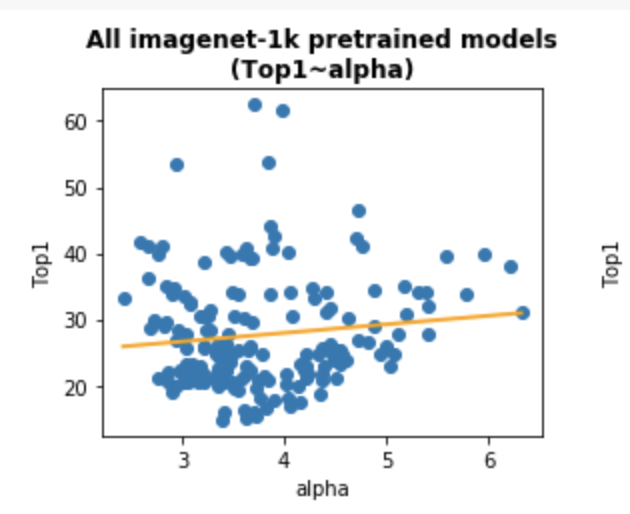
\includegraphics[width=2.5cm]{img/imagenet1k_alpha.png}
        \label{fig:imagenet1k-alpha}
    }
    \qquad
    \subfigure[ CIFAR 10 ]{
        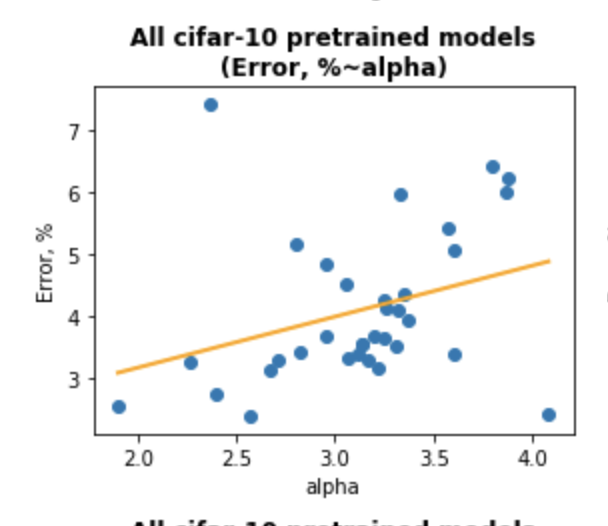
\includegraphics[width=2.5cm]{img/cifar10_alpha.png}
        \label{fig:cifar10.alpha}
    }
    \qquad
    \subfigure[ CIFAR 100 ]{
        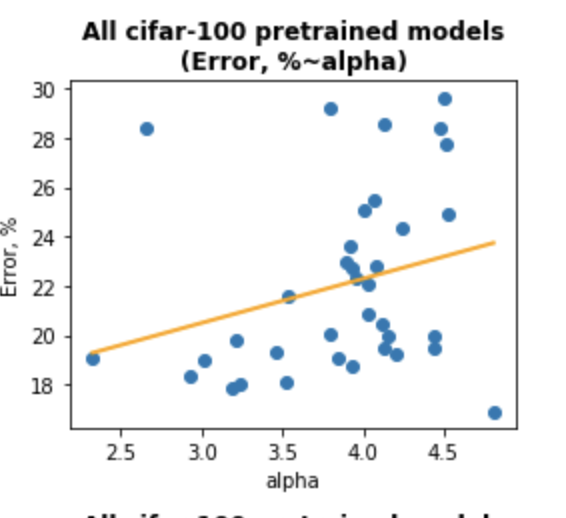
\includegraphics[width=2.5cm]{img/cifar100_alpha.png}
        \label{fig:cifar100.alpha}
    }
    \qquad
    \subfigure[ SVHN ]{
        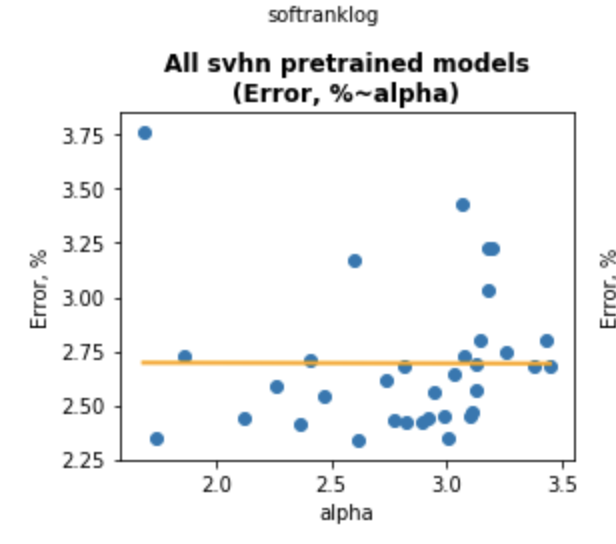
\includegraphics[width=2.5cm]{img/svhn_alpha.png}
        \label{fig:svhn.alpha}
    }
    \qquad
    \subfigure[ CUB 200 ]{
        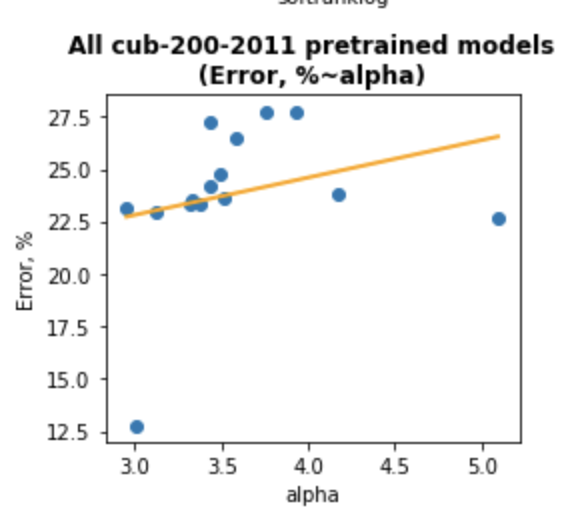
\includegraphics[width=2.5cm]{img/cub200_alpha.png}
        \label{fig:cub200.alpha}
    }
    \caption{\charles{Preliminary charts:} PL exponent $\alpha$ vs. reported Top1 Test Accuracies for pretrained DNNs available\charles{ref} for 5 different data sets.}

    \label{fig:DSalphas}
\end{figure}







\section{XXX: PLACEHOLDER STUFF PROBABLY TO BE REMOVED}

\subsection{XXX: PLACEHOLDER STUFF PROBABLY TO BE REMOVED}

\michael{I put this here for now as a placeholder.  Where to put it.  Maybe in a discussion/conclusion if there is space.}

\paragraph{XXX.}
XXX.  THIS VERIFICATION IS NOT ABOUT CONV LAYERS, IT IS ABOUT PL MORE GENERALLY, CORRECT?  WE SHOULD CLARIFY AND SQUISH.
To verify that our approach is meaningful, we need to confirm that the ESD is neither due to a random matrix, nor due to unsually large matrix elements, but, in fact, captures correlations learned from the data. 
We examine typical layer for the pretained AlexNet model (distributed with pyTorch). 
Figure~\ref{fig:alexnet1} displays the ESD for the first slice (or matrix $\mathbf{W}$) of the third Conv2D layer, extracted from a 4-index Tensor of shape $(384, 192, 3, 3)$.  The red line displays the best fit to a random matrix, using the Marchenko pastur theory~\cite{MM18_TR}.  We can see the random matrix model does not describe the ESD very well. For comparison, Figure \ref{fig:alexnet2} shows the ESD of the same matrix, randomly shuffled; here looks similar to the red line plot of the orginal ESD.  In fact, the empircal ESD is better modeled with a truncated power law distribtion.
\michael{We may want to give a one-sentence summary of this par and fig at the end of the previous par.}
\charles{Here, on the RMT MP stuff, I think it makes sense to point back}

\begin{figure}[H]
   \centering
   \subfigure[Actual ESD]{
     %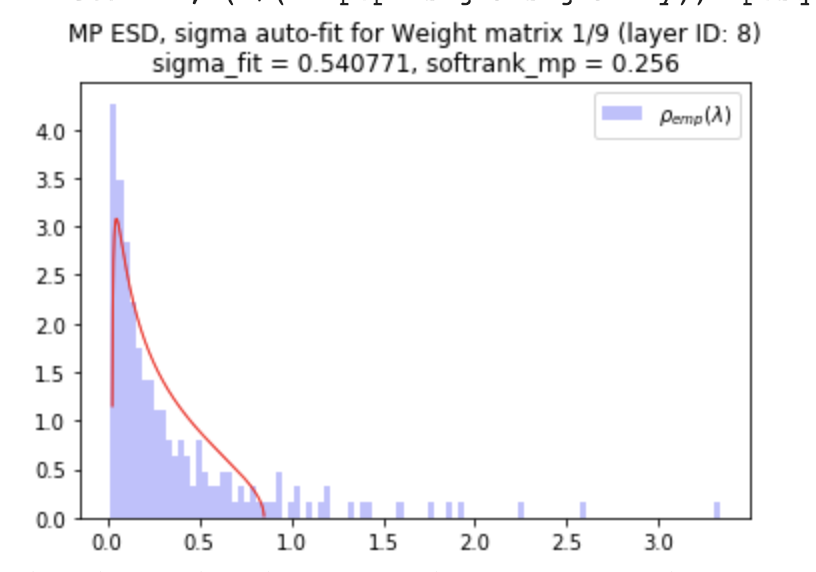
\includegraphics[scale=0.5]{img/alexnet1.png} 
     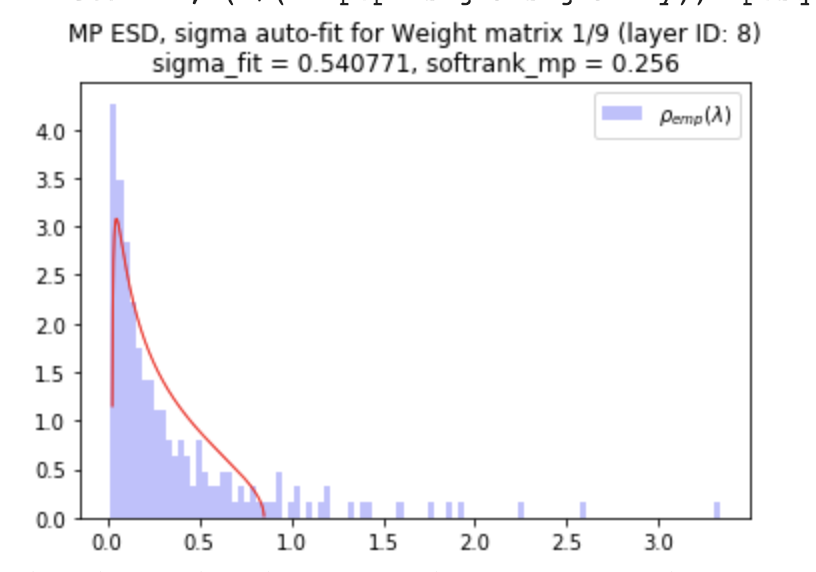
\includegraphics[scale=0.25]{img/alexnet1.png} 
     \label{fig:alexnet1}
   }
   \subfigure[ESD of randomly shuffled matrix]{
      %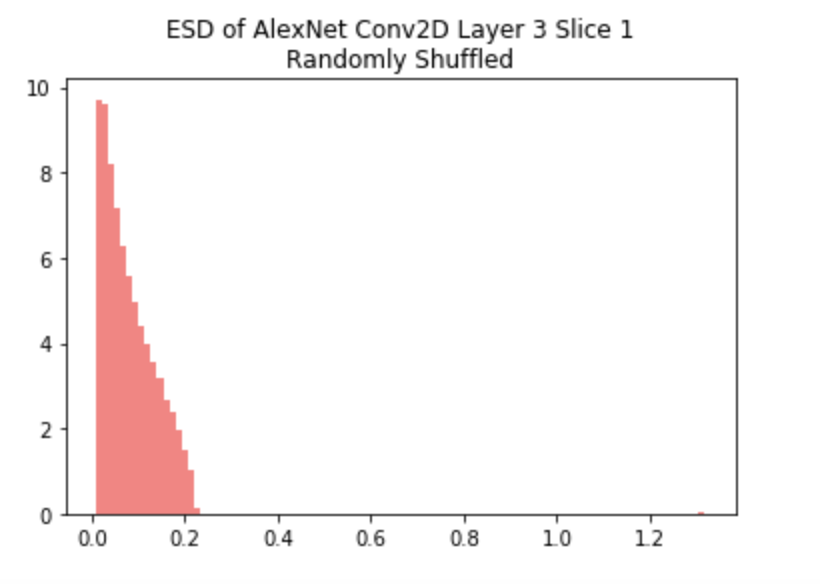
\includegraphics[scale=0.5]{img/alexnet2.png}
      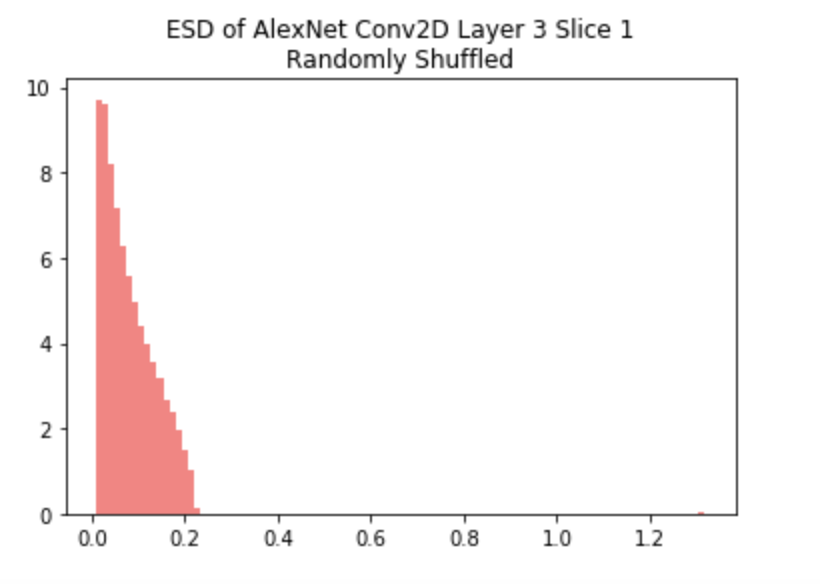
\includegraphics[scale=0.25]{img/alexnet2.png}
      \label{fig:alexnet2}
   }
   \caption{ESD of AlexNet Conv2D pre-Activation map for Layer 3 Slice 1, actual and randomized.
            \michael{Need better figs here.}
           }
   \label{fig:alexnet}
\end{figure}


Although the ESD is \emph{Heavy Tailed}, this does not imply that the orginal matrix $\mathbf{W}$ is itself heavy tailed--only the correlation matrix $\mathbf{X}$ is. 
If $\mathbf{W}$ was, then it would contain 1 or more unusually large matrix elements, and they would dominate the ESD.  
Of course the randomized $\mathbf{W}$ would also be heavy tailed, but its ESD neither resembles the original nor is it heavy tailed. 
So we can rule out $\mathbf{W}$ being heavy tailed.
\michael{These comments seem out of place, since they hold more generally than for the Conv2D layers.}
\charles{Agreed. We could move this up.  We have never really talked about this, but it is essential to explain the difference between assuming W is heavy tailed , which confuses everyone}

These plots tell us that the pre-activation maps of the Conv2D contains significant correlations learned from the data.  
By modeling the ESD with a power law distribution $\lambda^{\alpha}$, we can characterize the amount of correlation learned;
the smaller the exponent $\alpha$, the more correlation in the weight matrix. 
\michael{These comments seem out of place, since they hold more generally than for the Conv2D layers.}

\subsection{XXX: PLACEHOLDER STUFF PROBABLY TO BE REMOVED}

Some other comments that we need to weave into a narrative eventually after later sections are written:
\begin{itemize}
\item
GPT versus GPT2.
What happens when we don't have enough data?
This is the main question, and we can use out metrics to evaluate that, but we also get very different results for GPT versus GPT2.
\item
The spectral norm is a regularizer, used to distinguish good-better-best, not a quality metric.
For example, it can ``collapse,'' and for bad models we can have small spectral norm.
So, it isn't really a quality metric.
\item
One question that isn't obvious is whether regularization metrics can be used as quality metrics.
One might think so, but the answer isn't obviously yes.
We show that the answer is No.
A regularizer is designed to select a unique solution from a non-unique good-better-best.
Quality metrics can also distinguish good versus bad.
\item
(We should at least mention this is like the statistical thing where we evaluate which model is better, as oposed to asking if a given model is good, I forget the name of that.)
\item
There are cases where the model is bad but regularization metric doesn't tell you that.
Quality should be correlated in an empirical way.
Correlated with good-better-best; but also tell good-bad.
\item
Question: why not use regularier for quality?
Answer: A regularizer selects from a given set of degenerate models one which is nice or unique.
It doesn't tell good versus bad, i.e., whether that model class is any good.
\item
Thus, it isn't obvious that norm-based metrics should do well, and they don't in general.
\item
We give examples of all of these: bad data; defective data; and distill models in a bad way.
(Of course, bad data means bad model, at least indirectly, since the quality of the data affects the properties of the model.)
\item
We can select a model and change it, i.e., we don't just do hyperparameter fiddling.
\end{itemize}

